\section{Algorithm}\label{sec:algorithm}

\algrenewcommand\algorithmicrequire{\textbf{Input:}}
\algrenewcommand\algorithmicensure{\textbf{Output:}}

\begin{figure}
\centering
\begin{tikzpicture}[x=1cm,y=1cm,
    stage/.style={draw=ink2, fill=white, rounded corners=1.5pt, text width=9.2cm, align=left, font=\small, inner sep=4pt},
    io/.style={stage, fill=light!70},
    side/.style={draw=ink2, fill=blueI!7, rounded corners=1.5pt, text width=3.1cm, align=left, font=\small, inner sep=4pt}]
  \node[io] (in) at (0,0) {\textbf{Input}: pre-processed segments of fixes $(t,\varphi,\lambda,z)$ and their phase labels};
  \node[stage, below=0.35cm of in] (p0) {\textbf{Phase 0} (per flight): positions on the ellipsoid, departure $k^\dep_i$, states and heading in glide, values on the 5-s grid};
  \node[stage, below=0.35cm of p0] (p1) {\textbf{Phase 1} (per date): candidate pairs with a KD-tree on one point per minute; windows $W_{ij}$ (Lemma~\ref{lem:filter})};
  \node[stage, below=0.35cm of p1] (p2) {\textbf{Phase 2} (per pair): exact correspondences, contact $a_{ij}(t)$, delay $l^*(t)$};
  \node[stage, below=0.35cm of p2] (p3) {\textbf{Phase 3} (per pair): pair intervals (gaps $<g$ joined, duration $\ge\tau^*$)};
  \node[stage, below=0.35cm of p3] (p4) {\textbf{Phase 4} (per date): sweep over the events $\to$ configurations, episodes, blocks};
  \node[io, below=0.35cm of p4] (out) {\textbf{Output}: tables T1--T5 and labels on the phases};
  \foreach \a/\b in {in/p0, p0/p1, p1/p2, p2/p3, p3/p4, p4/out} \draw[->, ink2] (\a) -- (\b);
  \node[side, right=0.6cm of p2.east, anchor=west, yshift=-0.45cm] (cal) {\textbf{Calibration} (Section~\ref{sec:calibration}): null model, $\tau^*$, plateau of the parameters};
  \draw[->, blueI] (cal.west |- p2.east) -- (p2.east);
  \draw[->, blueI] (cal.south) |- (p3.east);
\end{tikzpicture}
\caption{The method as a pipeline. Phases 1--4 work date by date: flights of different days do not
interact, so the computation runs in parallel over the dates and needs the memory of one day.}
\label{fig:pipeline}
\end{figure}

\subsection{Phase 0: preparation per flight}\label{sec:phase0}

\begin{enumerate}[label=(\alph*), leftmargin=2em]
\item \textbf{Positions.} The Earth-centred position of every fix (Section~\ref{sec:data}). One
frame serves all the flights, at any distance and without a map projection, so the coordinates of
two flights compare directly.

\item \textbf{Altitude.} GNSS $z$, unchanged.

\item \textbf{Departure.} $k^\dep_i$ from~\eqref{eq:departure}.

\item \textbf{States and heading.} $s_i(k)$ from the phase labelling. In glide, $\vh_i(k)$ is the
direction of the horizontal velocity, filtered with Savitzky--Golay, in the east and north
directions of the fix itself. Two pilots compared by~\eqref{eq:heading} are less than
$\varepsilon_h$ apart, so their east and north directions differ by less than 0.01\textdegree.

\item \textbf{Grid.} The instants of $\Delta\Z$, with $\Delta=5$~s, the same for all flights. A
grid instant takes the position and the altitude of the fix at that instant or, between two fixes
of the same segment at most $h_{\max}=10$~s apart, the values interpolated linearly between them,
with the state and the heading of the nearer fix; elsewhere the flight has no position. On a
logger that records every second every grid instant is a fix. An interpolated position is at most
$v_{\max}h/2$ from the true one, for two fixes $h$ apart: 69~m at 5~s, 139~m at 10~s.
\end{enumerate}

\begin{doubt}{Is $\Delta=5$~s enough in a thermal?}
Four points per turn do not draw the spiral (Figure~\ref{fig:decimation}), but the contact does
not need its shape. What matters is how far a grid position can be from the track between two
grid instants, compared with the tolerances:
\begin{itemize}[leftmargin=1.2em, itemsep=1pt, topsep=2pt]
  \item horizontally, a pilot is never more than $v_{\max}\Delta/2\approx69$~m from the nearest
        grid point in the worst case, about 20~m while circling at 8~m/s; $\varepsilon_h=500$~m,
        and a whole thermal of radius 25~m fits in a small fraction of it;
  \item vertically, $w\Delta/2=5$~m at 2~m/s and at most 12.5~m at 5~m/s, against
        $\varepsilon_z=300$~m;
  \item on the delay, a grid of 5~s against the $\pm150$~s to which altitude resolves it in a
        thermal (Section~\ref{sec:roles});
  \item on the ends of the intervals, $\pm\Delta$ against $g=120$~s.
\end{itemize}
States and headings are computed on the fixes, before the grid, and lose nothing. The check of
Section~\ref{sec:checks} repeats the computation with $\Delta=1$~s on a subset of 1-Hz pairs.
\end{doubt}

\begin{figure}
\centering
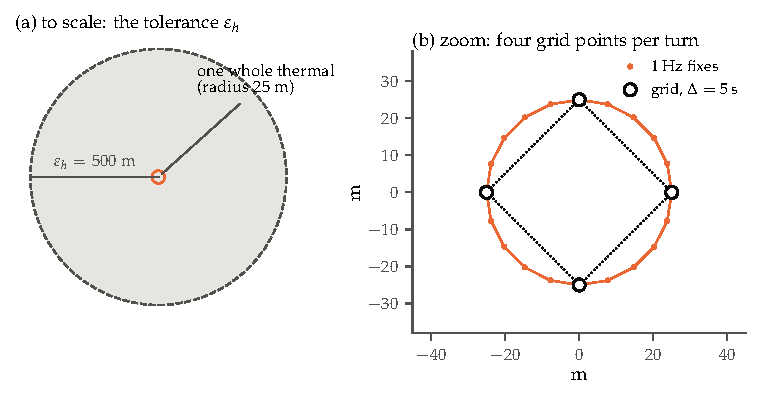
\includegraphics[width=0.92\textwidth]{figures/decimation.pdf}
\caption{The 5-s grid in a thermal, to scale. (a) The horizontal tolerance $\varepsilon_h$ and a whole
thermal of radius 25~m. (b) One turn of 20~s sampled at 1~Hz and on the grid of $\Delta=5$~s:
four grid points per turn, each within 20~m of the 1~Hz fixes around it.}
\label{fig:decimation}
\end{figure}

\begin{table}
\centering
\small
\begin{tabular}{@{}*{7}{l}@{}}
\toprule
\texttt{date} & \texttt{flight} & \texttt{t} & \texttt{X, Y, Z} & \texttt{z} & \texttt{ve, vn} & \texttt{state} \\
\midrule
partition & int32 & int32 (s) & float32 & float32 & float16 & int8 \\
\bottomrule
\end{tabular}
\caption{Table of the grid points, in Parquet partitioned by date: about 30 bytes per row.
\texttt{X, Y, Z} are the Earth-centred position, to 0.5~m in float32; \texttt{ve, vn} the unit
heading in the east and north of the point.}
\label{tab:points}
\end{table}

Under the assumption, to be checked, of $1.86\times10^5$ flights lasting 1.5~h on average, the
table has about $2\times10^8$ rows: 6~GB uncompressed, less in Parquet. It is worth keeping,
because the null model and the calibration read it several times.

\subsection{Phase 1: candidate pairs}\label{sec:phase1}

The exact computation over all pairs of simultaneous flights is wasted effort: almost all of them
never come close. A coarse filter reduces the pairs, with the guarantee of losing none.

The filter works on segments. Let $\tilde\x_i(s)$ be a segment of flight $i$ extended by holding
its first position before it and its last position after it, and let $v_{\max}$ be the top speed
of the pre-processing: within a segment no step between two fixes is faster, because the
excursion rule (step~6) deletes or splits at any faster step, and the interpolation onto the grid
keeps the bound. The filter compares positions at whole minutes, and a minute may fall just before
or just after a segment: the extension gives the track a position there.

\begin{lemma}[no false negative]\label{lem:filter}
If $(t,t')\in\M_{ij}$, $\tilde\x_i$ and $\tilde\x_j$ are the extended segments that contain $t$
and $t'$, and $t_c=60\cdot\mathrm{round}(t/60)$, then
\begin{equation}\label{eq:filter}
  \|\tilde\x_i(t_c)-\tilde\x_j(t_c)\| \le D_c := \varepsilon_h+v_{\max}\,(\delta+60~\mathrm{s}).
\end{equation}
\end{lemma}

\begin{inwords}
$t_c$ is the whole minute nearest to $t$ (Figure~\ref{fig:lemma}a), and both positions
in~\eqref{eq:filter} are read at that \emph{same} instant. If two pilots have a correspondence at
all, then at the nearest whole minute they are less than $D_c$ apart; a pair farther than $D_c$ at
every minute has no correspondence and can be discarded.
\end{inwords}

\begin{proof}
The extension with a fixed position keeps the Lipschitz property
$\|\tilde\x(s)-\tilde\x(s')\|\le v_{\max}|s-s'|$ for all $s,s'$. By construction of $t_c$,
$|t-t_c|\le30$~s, and $|t'-t_c|\le|t'-t|+|t-t_c|\le\delta+30$~s. The triangle inequality along
the path $\tilde\x_i(t_c)\to\x_i(t)\to\x_j(t')\to\tilde\x_j(t_c)$ (Figure~\ref{fig:lemma}) gives
\begin{align*}
  \|\tilde\x_i(t_c)-\tilde\x_j(t_c)\|
  &\le \|\tilde\x_i(t_c)-\x_i(t)\| + \|\x_i(t)-\x_j(t')\| + \|\x_j(t')-\tilde\x_j(t_c)\|\\
  &\le 30\,v_{\max} + \varepsilon_h + v_{\max}(\delta+30),
\end{align*}
where the middle term is below $\varepsilon_h$ because $(t,t')$ is a correspondence
(Definition~\ref{def:correspondence}).
\end{proof}

\begin{figure}
\centering
\begin{tikzpicture}[x=1cm,y=1cm]
  \begin{scope}
    \node[panel] at (0,2.0) {(a) the nearest minute};
    \draw[->, ink2] (0,0) -- (9.6,0) node[right, lbl, ink] {$t$ (s)};
    \foreach \x/\l in {0/0, 3/60, 6/120, 9/180} {\draw[ink, line width=0.8pt] (\x,-0.1) -- (\x,0.1); \node[lbl, below] at (\x,-0.1) {\l};}
    \fill[blueI!15] (1.5,0.18) rectangle (4.5,0.45);
    \node[note] at (3.0,0.65) {rounded to 60};
    \fill[orangeJ!15] (4.5,0.18) rectangle (7.5,0.45);
    \node[note] at (6.0,0.65) {rounded to 120};
    \fill[ink] (4.45,0) circle (1.6pt); \node[lbl] (n89) at (3.9,1.25) {$t=89$};
    \draw[->, ink2] (n89) -- (4.43,0.08);
    \fill[ink] (4.55,0) circle (1.6pt); \node[lbl] (n91) at (5.1,1.25) {$t=91$};
    \draw[->, ink2] (n91) -- (4.57,0.08);
    \node[note, anchor=west, align=left] at (9.9,0.5) {$|t-t_c|\le30$~s\\$|t'-t_c|\le\delta+30$~s};
  \end{scope}
  \begin{scope}[shift={(1.5,-3.3)}]
    \node[panel] at (-1.5,2.0) {(b) the chain of the proof};
    \coordinate (a) at (0.2,0.2); \coordinate (b) at (1.6,1.0); \coordinate (c) at (3.0,1.25); \coordinate (d) at (6.4,0.5);
    \draw[blueI, line width=1pt] (a) -- node[above left=-2pt, lbl] {$\le30\,v_{\max}$} (b);
    \draw[ink, line width=1pt] (b) -- node[above, lbl] {$<\varepsilon_h$} (c);
    \draw[orangeJ, line width=1pt] (c) -- node[above right=-2pt, lbl] {$\le(\delta+30)\,v_{\max}$} (d);
    \draw[ink2, densely dashed] (a) -- node[below, lbl] {$\le D_c$} (d);
    \node[pt i] at (a) {}; \node[pt i] at (b) {}; \node[pt j] at (c) {}; \node[pt j] at (d) {};
    \node[lbl, left] at (a) {$\tilde\x_i(t_c)$};
    \node[lbl, above] at (b) {$\x_i(t)$};
    \node[lbl, above] at (c) {$\x_j(t')$};
    \node[lbl, right] at (d) {$\tilde\x_j(t_c)$};
  \end{scope}
\end{tikzpicture}
\caption{Lemma~\ref{lem:filter}. (a) Every instant is at most 30~s from its nearest whole minute.
(b) From $i$ at the minute to $j$ at the same minute through the correspondence $(t,t')$: each step
is bounded by the time it takes at most $v_{\max}$, or by $\varepsilon_h$.}
\label{fig:lemma}
\end{figure}

With $v_{\max}=100$~km/h, $\delta=300$~s and $\varepsilon_h=500$~m, $D_c\approx10.5$~km. The
filter runs as follows, for each date.
\begin{enumerate}
  \item For each segment keep one point per minute of its extended track, for $t_c$ from
        $\delta+60$~s before its first instant after the departure to $\delta+60$~s after its
        last instant. This is the interval in which the lemma may ask for the position, whichever
        of the two roles the flight has.
  \item Build a single KD-tree~\cite{virtanen2020} on the coordinates $(X, Y, Z, K t_c/60)$ with
        $K\gg D_c$, for example $K=10^8$~m: points of different minutes are more than $D_c$ apart
        and are never paired (Figure~\ref{fig:kdtree}).
  \item The search of all pairs within $D_c$ (\texttt{query\_pairs}) returns pairs of points of
        the same minute, hence triples $(i,j,t_c)$; the pairs of two segments of the same flight
        are dropped.
  \item For each candidate pair, with $i<j$, the window is
        $W_{ij}=\bigcup_{t_c}[t_c-30,t_c+30]\cap T^\dep_i$, the union over the minutes $t_c$ at which
        the pair passed the filter: a set of instants of the flight of $i$.
\end{enumerate}
By the lemma, every correspondence $(t,t')\in\M_{ij}$ has $t\in W_{ij}$. The cost is
$O(n_d\log n_d)$ per date, with $n_d$ the number of points per minute of the day. Phase~1 is worth
running on the whole dataset before Phase~2: the number of pairs and the total duration of the
windows give a precise estimate of the cost that follows.

\begin{figure}
\centering
\begin{tikzpicture}[x=1cm,y=1cm]
  \foreach \k/\h in {0/12{:}00, 1/12{:}01, 2/12{:}02} {
    \begin{scope}[shift={(0,1.55*\k)}]
      \fill[light!70] (0,0) -- (4.2,0) -- (5.4,0.9) -- (1.2,0.9) -- cycle;
      \draw[ink2, line width=0.4pt] (0,0) -- (4.2,0) -- (5.4,0.9) -- (1.2,0.9) -- cycle;
      \node[lbl, anchor=west] at (5.5,0.45) {$t_c=$ \h, fourth coordinate $K t_c/60$};
    \end{scope}
  }
  \foreach \p in {(1.2,0.3),(2.0,0.55),(3.3,0.4),(4.4,0.6)} \fill[ink] \p circle (1.5pt);
  \foreach \p in {(1.0,1.85),(2.1,2.2),(2.5,2.05),(3.9,2.0),(4.6,2.3)} \fill[ink] \p circle (1.5pt);
  \foreach \p in {(1.6,3.4),(2.9,3.6),(3.6,3.45)} \fill[ink] \p circle (1.5pt);
  \draw[blueI, line width=0.8pt] (2.3,2.12) ellipse (0.75 and 0.33);
  \node[lbl, blueI, anchor=west] at (-1.5,2.75) {ball of radius $D_c$};
  \draw[blueI] (-0.1,2.7) -- (1.7,2.25);
  \draw[<->, ink2] (-0.4,0.45) -- node[left, lbl] {$K\gg D_c$} (-0.4,2.0);
\end{tikzpicture}
\caption{The KD-tree of Phase~1. Each minute is a layer of the space $(X,Y,Z,Kt_c/60)$, drawn
here as a plane, and the layers are $K\gg D_c$ apart: a search of radius $D_c$ only finds points of the same minute, so one
tree does the work of one search per minute.}
\label{fig:kdtree}
\end{figure}

\subsection{Phase 2: exact correspondences}\label{sec:phase2}

\begin{lemma}\label{lem:scan}
Scanning the instants $t\in W_{ij}$ and the delays $l\in\Lambda=\{-L\Delta,\dots,L\Delta\}$, with
$L=\lfloor\delta/\Delta\rfloor$, enumerates all pairs of $\M_{ij}$; hence $m_{ij}$ and $m_{ji}$ are
obtained exactly.
\end{lemma}

\begin{proof}
Every $(t,t')\in\M_{ij}$ has $t\in W_{ij}$ (Lemma~\ref{lem:filter}) and $t'-t\in\Lambda$. Moreover
$m_{ji}(t')=1$ if and only if there is a $t$ with $(t,t')\in\M_{ij}$, and every such $t$ lies in
$W_{ij}$.
\end{proof}

\begin{algorithm}[htbp]
\caption{Phase 2: scan of one candidate pair}\label{alg:scan}
\begin{algorithmic}[1]
\Require flights $i<j$, on the grid; window $W\subseteq T^\dep_i$; delays $\Lambda$
\Ensure contact $a$ on the support $W\cup(W+\Lambda)$; delay $l^*$ on $W$
\State $m_{ij}\gets0$;\ $m_{ji}\gets0$;\ $d^{\min}\gets+\infty$;\ $l^*\gets$ undefined
\For{$l\in\Lambda$}
  \State $\tau\gets\{t\in W:\ t+l\in T^\dep_j\}$ \Comment{array of instants}
  \State $d\gets\|\x_i(\tau)-\x_j(\tau+l)\|$;\ $h\gets|z_i(\tau)-z_j(\tau+l)|$
  \State $c\gets(d<\varepsilon_h)\wedge(h<\varepsilon_z)\wedge D_{ij}(\tau,\tau+l)$
  \State $m_{ij}[\tau]\gets m_{ij}[\tau]\vee c$;\ $m_{ji}[\tau+l]\gets m_{ji}[\tau+l]\vee c$
  \State $u\gets c\wedge(d<d^{\min}[\tau])$;\ $d^{\min}[\tau]\gets d$ and $l^*[\tau]\gets l$ where $u$
\EndFor
\State $a(t)\gets m_{ij}(t)\vee m_{ji}(t)$
\State \Return $a$, $l^*$
\end{algorithmic}
\end{algorithm}

Each pass of the loop takes one delay $l$: in the $(t,t')$ plane it is the diagonal $t'=t+l$,
evaluated over the whole window at once (Figure~\ref{fig:scan}). The cost is
$\sum_{\rm pairs}|W_{ij}|\,(2L+1)$ distance evaluations, with $2L+1=121$ for $\delta=5$~min and
$\Delta=5$~s. The memory is $O(|W_{ij}|)$ per pair: boolean arrays are accumulated, without
generating the list of pairs of points. Each step of the loop is a vector operation on arrays.

\begin{figure}
\centering
\begin{tikzpicture}[x=0.55cm,y=0.55cm]
  \fill[light] (0,0) -- (3,0) -- (12,9) -- (12,12) -- (9,12) -- (0,3) -- cycle;
  \fill[blueI!14] (2,0) rectangle (4.5,12);
  \fill[blueI!14] (6.5,0) rectangle (9,12);
  \foreach \l in {-3,-2.5,...,3} {
    \draw[ink2!70, line width=0.3pt] ({max(2,-1*\l)},{max(2,-1*\l)+\l}) -- ({min(4.5,12-\l)},{min(4.5,12-\l)+\l});
    \draw[ink2!70, line width=0.3pt] ({max(6.5,-1*\l)},{max(6.5,-1*\l)+\l}) -- ({min(9,12-\l)},{min(9,12-\l)+\l});
  }
  \draw[orangeJ, line width=1.4pt] (2,3.5) -- (4.5,6.0);
  \draw[orangeJ, line width=1.4pt] (6.5,8.0) -- (9,10.5);
  \draw[muted, densely dashed] (0,0) -- (12,12);
  \draw[->, ink2] (0,0) -- (12.8,0) node[right, lbl, ink] {$t$};
  \draw[->, ink2] (0,0) -- (0,12.8) node[above, lbl, ink] {$t'$};
  \draw[decorate, decoration={brace, mirror, amplitude=4pt}, blueI] (2,-0.2) -- (4.5,-0.2);
  \draw[decorate, decoration={brace, mirror, amplitude=4pt}, blueI] (6.5,-0.2) -- (9,-0.2);
  \node[lbl, below=6pt] at (5.5,-0.2) {$W_{ij}$};
  \node[note, anchor=west, align=left] at (13.2,9.2) {orange: one pass of the loop,\\a fixed delay $l$ over all of $W_{ij}$};
  \node[note, anchor=west, align=left] at (13.2,6.4) {grey lines: the $2L+1$ delays of $\Lambda$};
  \node[note, anchor=west, align=left] at (13.2,4.0) {grey band: $|t'-t|\le\delta$};
\end{tikzpicture}
\caption{Phase 2 in the $(t,t')$ plane. Only the columns of the window $W_{ij}$ are scanned, one
diagonal $t'=t+l$ at a time; by Lemma~\ref{lem:scan} this covers all of $\M_{ij}$.}
\label{fig:scan}
\end{figure}

\subsection{Phase 3: pair intervals}\label{sec:phase3}

From the contact $a$ one extracts the runs of 1, joins those separated by gaps shorter than $g$
and keeps those lasting at least $\tau^*$ (Definition~\ref{def:pair-interval}). For each interval one also records:
\begin{itemize}
  \item the signed median delay $\ell_{\rm med}=\mathrm{median}\{l^*(t):\ t\in[t_{\rm on},t_{\rm
        off}),\ m_{ij}(t)=1\}$: if $\ell_{\rm med}>0$, $j$ follows $i$, as in~\cite{li2013}. In a
        search the delay is poorly determined (Section~\ref{sec:roles}), so the instants at which
        either pilot is in \st{search} are better left out of the median;
  \item the distance between the takeoffs $d_{\rm dec}=\|\x_i(k^0_i)-\x_j(k^0_j)\|$, which allows
        requirement (R1) to be imposed afterwards, if wanted.
\end{itemize}

\subsection{Phase 4: configurations and episodes}\label{sec:phase4}

Between one event and the next the set of active edges does not change, so it is enough to update
the components at the instants at which an interval starts or ends, and only around the nodes
involved (Figure~\ref{fig:sweep}).

\begin{algorithm}[htbp]
\caption{Phase 4: sweep over the events of one day}\label{alg:sweep}
\begin{algorithmic}[1]
\Require pair intervals $\I$ of the day
\Ensure configurations; episodes (classes of a union--find)
\State events $\gets\{(t_{\rm on},+,\{a,b\}),\ (t_{\rm off},-,\{a,b\})\}$ sorted in time
\State $A\gets\emptyset$ (active edges);\ $\mathcal{O}\gets\emptyset$ (open configurations)
\For{each instant $t_e$, with its batch of events $B$}
  \State $U\gets$ endpoints of the edges in $B$ \Comment{nodes involved}
  \State $R\gets U\cup\bigcup\{M_c:\ c\in\mathcal{O},\ M_c\cap U\ne\emptyset\}$
  \State update $A$ with the events of $B$
  \State $\mathcal{K}\gets$ connected components of $(R, A|_R)$ with at least two nodes \Comment{local visit}
  \State $X\gets\{c\in\mathcal{O}:\ M_c\subseteq R,\ M_c\notin\mathcal{K}\}$; close every $c\in X$ with $t^{\rm end}_c\gets t_e$
  \For{$K\in\mathcal{K}$ that is not already an open configuration}
    \State open $c'$ with $M_{c'}=K$ and $t^{\rm start}_{c'}=t_e$
    \For{$c\in X$ with $M_c\cap K\ne\emptyset$}
      \State \Call{Union}{$c, c'$}
    \EndFor
  \EndFor
\EndFor
\end{algorithmic}
\end{algorithm}

\begin{lemma}\label{lem:local}
After the update, the connected component of every node of $R$ is contained in $R$; hence the
local recomputation of Algorithm~\ref{alg:sweep} gives the same components as a global one.
\end{lemma}

\begin{proof}
Before the update the open configurations are disjoint, and those that touch $U$ lie entirely in
$R$. A path that starts in $R$ uses old edges, which stay inside the old component, or new edges,
whose endpoints lie in $U\subseteq R$. By induction on the length of the path, every node it
reaches is in $R$.
\end{proof}

\begin{figure}
\centering
\begin{tikzpicture}[x=1cm,y=1cm]
  \foreach \sx/\new in {0/0, 7.2/1} {
    \begin{scope}[shift={(\sx,0)}]
      \ifnum\new=1 \fill[blueI!10, rounded corners=10pt] (-0.45,-0.5) rectangle (3.85,2.5); \fi
      \coordinate (a) at (0,0.5); \coordinate (b) at (0.9,1.8); \coordinate (c) at (1.6,0.4);
      \coordinate (d) at (2.6,1.7); \coordinate (e) at (3.4,0.6);
      \coordinate (f) at (4.8,1.6); \coordinate (g) at (5.5,0.5);
      \draw[edge] (a) -- (b) -- (c);
      \draw[edge] (d) -- (e);
      \draw[edge] (f) -- (g);
      \ifnum\new=1 \draw[edge, orangeJ, line width=1.8pt] (c) -- (d); \fi
      \foreach \n in {a,b,c,d,e} \node[flight] at (\n) {};
      \node[flight, fill=light] at (f) {}; \node[flight, fill=light] at (g) {};
    \end{scope}
  }
  \node[lbl] at (1.7,2.85) {before $t_e$};
  \node[lbl] at (8.9,2.85) {at $t_e$: a new edge (orange)};
  \node[note, anchor=north, align=center] at (8.9,-0.6) {$R$ (shaded): the endpoints of the new edge\\and the open configurations they belong to};
  \node[note, anchor=south, align=center] at (12.35,2.15) {untouched};
  \draw[->, muted, line width=0.8pt] (5.9,1.0) -- (6.8,1.0);
\end{tikzpicture}
\caption{One step of the sweep. Only the nodes of $R$ are visited again; the grey component far
away keeps its configuration. The animation of Figure~\ref{fig:day} runs the sweep over a whole
day.}
\label{fig:sweep}
\end{figure}

The cost per day is $O(|\I|\log|\I|)$ for the sorting, plus the sum of the sizes of the
components involved at each event, at most a few hundred nodes. The classes of the
union--find~\cite{tarjan1975} are the episodes. From the list of the configurations one obtains
$\gamma_i(t)$ as in~\eqref{eq:membership}, filling with \st{S} the stretches after the departure
not covered by a configuration and with \st{L} the local phase.

\subsection{Costs and space}\label{sec:costs}

\begin{table}
\centering
\small
\begin{tabular}{@{}l l l@{}}
\toprule
Phase & Cost & Data produced \\
\midrule
0 & linear in the number of fixes ($\sim10^9$) & grid points, $\sim2\times10^8$ rows \\
1 & $O(n_d\log n_d)$ per date, $\sum_d n_d\sim1.7\times10^7$ & candidate pairs and windows \\
2 & $\sum|W_{ij}|(2L+1)$; measured after Phase~1 & temporary arrays per pair \\
3 & linear in the duration of the windows & T1, pair intervals \\
4 & $O(|\I|\log|\I|)$ per date & T2--T5 \\
\bottomrule
\end{tabular}
\caption{Costs and space. The numbers assume $1.86\times10^5$ flights of 1.5~h on average and are
to be checked on the data.}
\label{tab:costs}
\end{table}

Phases 1--4 are independent across dates and run in parallel without coordination. Phase~2
dominates the cost; Phase~1 allows it to be estimated before running it.
